% This template mostly comes from Jiayi Weng. 
% And his Page is here:
%   https://github.com/Trinkle23897/THU-Beamer-Theme

% The lateset HHU-Beamer-Theme is modified by Hu Lihan.
% The source codes of this latex file for HHU can be found here:
% https://github.com/MartinHu1997/HHU-Beamer-Theme.git
%-------------------------------------------------------------

\documentclass{beamer}
%\usepackage{ctex, hyperref}
\usepackage{ctex, hyperref, fontspec}  % 支持中文及不同字体设置
\usepackage[T1]{fontenc}

% 设置中文和英文的字体
\setCJKmainfont{Microsoft YaHei}  % 设置中文字体为微软雅黑
\setmainfont{Times New Roman}  % 设置英文字体为Times New Roman

% other packages
\usepackage{latexsym,amsmath,xcolor,multicol,booktabs,calligra}
\usepackage{graphicx,pstricks,listings,stackengine}
\usepackage{HHU_beamer}

\author{解奥南 \and xxx}
\title{分布式智能医疗系统中轻量级、匿名的医疗大数据互认证方案}
%\subtitle{学术汇报 Latex}
\institute{
  %\inst{1}
  河海大学 计算机与软件学院
}
\date{2024年11月2日}


% defs
\def\cmd#1{\texttt{\color{red}\footnotesize $\backslash$#1}}
\def\env#1{\texttt{\color{blue}\footnotesize #1}}
\definecolor{deepblue}{rgb}{0,0,0.5}
\definecolor{deepred}{rgb}{0.6,0,0}
\definecolor{deepgreen}{rgb}{0,0.5,0}
\definecolor{halfgray}{gray}{0.55}

\lstset{
    basicstyle=\ttfamily\small,
    keywordstyle=\bfseries\color{deepblue},
    emphstyle=\ttfamily\color{deepred},    % Custom highlighting style
    stringstyle=\color{deepgreen},
    numbers=left,
    numberstyle=\small\color{halfgray},
    rulesepcolor=\color{red!20!green!20!blue!20},
    frame=shadowbox,
}


\begin{document}

%\kaishu
\begin{frame}
    \titlepage
    \begin{figure}[htpb]
        \begin{center}
            
\includegraphics[width=0.35\linewidth]{pic/HHU_logo.png}
        \end{center}
    \end{figure}
\end{frame}

\begin{frame}
    \tableofcontents[sectionstyle=show,subsectionstyle=show/shaded/hide,subsubsectionstyle=show/shaded/hide]
\end{frame}


\section{引言}

\begin{frame}{大数据技术的发展背景}
    \textbf{1. 大数据技术的发展背景}:
    \begin{itemize}
        \item “大数据”是需要新的处理模式才能具有更强的决策力、洞察发现力和流程优化能力来适应海量、高增长率和多样化的信息资产。
    \end{itemize}

    % 使用 \resizebox 调整表格大小,并使用三线表格式
    \begin{table}[ht]
        \centering
        \resizebox{\textwidth}{!}{  % 自动调整表格宽度以适应幻灯片页面
        \begin{tabular}{l l}  % 第一列和第二列都左对齐
            \toprule
            \multicolumn{1}{c}{\textbf{特征}} & \multicolumn{1}{c}{\textbf{介绍}} \\  % 只让表头居中
            \midrule
            容量 (Volume) & 数据的大小决定所考虑的数据的价值和潜在的信息 \\
            种类 (Variety) & 数据类型的多样性 \\
            速度 (Velocity) & 指获得数据的速度 \\
            可变性 (Variability) & 妨碍了处理和有效地管理数据的过程 \\
            真实性 (Veracity) & 数据的质量 \\
            复杂性 (Complexity) & 数据量巨大,来源多渠道 \\
            价值 (Value) & 合理运用大数据,以低成本创造高价值 \\
            \bottomrule
        \end{tabular}
        }
        \caption{大数据的特征}
    \end{table}
    

    
\end{frame}

% \begin{frame}[allowframebreaks]{大数据在智能医疗中的作用}
%     % 文字部分
%     \textbf{2. 大数据在智能医疗中的作用:}
    
%     \vspace{0.3cm}
%     分布式智能医疗是指通过集成各种智能医疗设备和通信网络,形成一个统一的基础设施,以实现系统的智能化、自动化和智能化管理。

%     \vspace{0.3cm}
%     分布式智能医疗中的大数据是指采用智能医疗技术所产生的海量医疗数据。医疗大数据的主要来源是组成分布式医疗网络的大量互联智能设备。
    
%     \vspace{0.3cm}
%     \begin{itemize}
%         \item 1. 医疗成像设备;
%         \item 2. 电子健康记录 (EHR) 系统;
%         \item 3. 医疗物联网 (IoMT) 设备;
%         \item 4. 临床运营管理系统;
%         \item 5. 供应链管理系统;
%         \item 6. 患者参与平台;
%     \end{itemize}
    
%     \vspace{0.3cm}
%     这些设备和系统在医疗网络中生成和传输大量数据,为医疗专业人员提供了深入的洞察力,以改善患者的治疗效果和医疗系统的运营效率。随着技术的发展,更多的智能设备将被集成到医疗网络中,进一步扩大医疗大数据的来源。
% \end{frame}

\begin{frame}{大数据在智能医疗中的作用 (1/2)}
    % 文字部分
    \textbf{2. 大数据在智能医疗中的作用:}
    
    \vspace{0.3cm}
    分布式智能医疗是指通过集成各种智能医疗设备和通信网络,形成一个统一的基础设施,以实现系统的智能化、自动化和智能化管理。

    \vspace{0.3cm}
    分布式智能医疗中的大数据是指采用智能医疗技术所产生的海量医疗数据。医疗大数据的主要来源是组成分布式医疗网络的大量互联智能设备。
    
    \vspace{0.3cm}
    \begin{itemize}
        \item 1. 医疗成像设备;
        \item 2. 电子健康记录 (EHR) 系统;
        \item 3. 医疗物联网 (IoMT) 设备;
    \end{itemize}
\end{frame}
\begin{frame}{大数据在智能医疗中的作用 (2/2)}
    \begin{itemize}
        \item 4. 临床运营管理系统;
        \item 5. 供应链管理系统;
        \item 6. 患者参与平台;
    \end{itemize}
    
    \vspace{0.3cm}
    这些设备和系统在医疗网络中生成和传输大量数据,为医疗专业人员提供了深入的洞察力,以改善患者的治疗效果和医疗系统的运营效率。随着技术的发展,更多的智能设备将被集成到医疗网络中,进一步扩大医疗大数据的来源。
\end{frame}


% \begin{frame}{医疗大数据技术的安全挑战}
%     \small  % 调整字体为较小的样式
    
%     \textbf{3. 医疗大数据技术的安全挑战:}
    
%     % 调整段落间距
%     \vspace{0.2cm}
%     分布式智能医疗网络主要由嵌入IoT设备、传感器、执行器、处理单元等的互联智能设备组成。分布式框架将大数据配置为多个系统,以减少单个系统的工作量。然而,更多的系统最终会带来更多的安全问题。
    
%     \vspace{0.2cm}
%     此外,\textbf{大多数用于大数据分析的工具都是在没有考虑数据安全问题的情况下开发的}。因此,对医疗大数据系统的攻击可能会破坏整个医疗系统的工作流程。未经授权的用户或设备可以访问和更改这些医疗保健数据,还可以控制连接到患者身体的IoT设备,这可能会给患者造成严重的医疗保健相关问题。
    
%     \vspace{0.2cm}
%     因此,需要依靠网络安全来保护医疗保健大数据,防止整个基础设施遭到破坏。医疗保健大数据的安全性可以通过维持CIA三要素来确保,即保密性、完整性和可用性。保密性意味着防止未经授权的数据访问或未经授权的数据披露。完整性防止未授权的数据修改,可用性确保数据在需要时始终可用。这些方面可以通过控制对医疗保健大数据的访问并确保对每个通信实体进行身份验证来实现。因此,在开发医疗基础设施的同时,有必要同时预先考虑所有三个安全方面。
% \end{frame}

\begin{frame}{医疗大数据技术的安全挑战 (1/2)}
    \small  % 调整字体为较小的样式
    
    \textbf{3. 医疗大数据技术的安全挑战:}
    
    % 调整段落间距
    \vspace{0.2cm}
    分布式智能医疗网络主要由嵌入IoT设备、传感器、执行器、处理单元等的互联智能设备组成。分布式框架将大数据配置为多个系统,以减少单个系统的工作量。然而,更多的系统最终会带来更多的安全问题。
    
    \vspace{0.2cm}
    此外,\textbf{大多数用于大数据分析的工具都是在没有考虑数据安全问题的情况下开发的}。因此,对医疗大数据系统的攻击可能会破坏整个医疗系统的工作流程。未经授权的用户或设备可以访问和更改这些医疗保健数据,还可以控制连接到患者身体的IoT设备,这可能会给患者造成严重的医疗保健相关问题。
\end{frame}

\begin{frame}{医疗大数据技术的安全挑战 (2/2)}
    \small  % 调整字体为较小的样式
    
    \textbf{4. 如何应对医疗大数据的安全挑战:}
    
    % 调整段落间距
    \vspace{0.2cm}
    因此,需要依靠网络安全来保护医疗保健大数据,防止整个基础设施遭到破坏。医疗保健大数据的安全性可以通过维持CIA三要素来确保,即保密性、完整性和可用性。保密性意味着防止未经授权的数据访问或未经授权的数据披露。
    
    \vspace{0.2cm}
    完整性防止未授权的数据修改,可用性确保数据在需要时始终可用。这些方面可以通过控制对医疗保健大数据的访问并确保对每个通信实体进行身份验证来实现。因此,在开发医疗基础设施的同时,有必要同时预先考虑所有三个安全方面。
\end{frame}




% \begin{frame}{问题背景}
%     \begin{itemize}
%         \item \textbf{医疗大数据的安全性问题}:在分布式智能医疗系统中,物联网(IoT)设备和传感器生成的医疗数据面临未经授权用户非法访问和篡改的风险,可能导致患者的医疗数据被篡改,进而影响患者的生命安全
%         \item \textbf{现有数据分析工具的安全性不足}:许多用于大数据分析的工具在开发时并未充分考虑数据的安全问题,导致医疗系统容易遭受网络攻击,整个医疗基础设施的工作流程可能因此受到干扰
%     \end{itemize}
% \end{frame}

% \begin{frame}{研究目标和动机}
%     \begin{itemize}
%         \item \textbf{研究目标}:设计一个轻量级的双向身份验证方案,确保分布式智能医疗系统中用户和设备的安全通信,抵御多种网络攻击。
%         \item \textbf{动机}:现有的验证方案在处理分布式智能医疗系统中的安全威胁时,无法兼顾资源受限设备的需求和应对复杂攻击的能力​
%     \end{itemize}
% \end{frame}

% \begin{frame}{研究问题}
%     \begin{itemize}
%         \item 如何确保医疗大数据的安全传输和访问?
%         \item 如何设计适用于资源受限设备的轻量级身份验证方案?
%         \item 如何抵御多种安全攻击?
%         \item 如何在保证安全的同时保护用户隐私?
%     \end{itemize}
% \end{frame}

\section{问题与相关工作}
\begin{frame}{问题与相关工作}
    \footnotesize  % 使用较小字体
    
    % 第一段内容
    为了维护安全,管理员需要对所有用户和设备进行注册。在开始新的会话之前,医生(用户)和 IoT 传感器节点(设备)相互验证,然后进行密钥交换。

    % 控制段落间距
    \vspace{0.2cm}
    
    % 第二段内容
    在支持批量的医疗保健系统中,有效的访问控制机制必须确保真实用户或设备不能访问医疗保健数据,除非他/她被授权访问。然而,访问控制模型的强度主要取决于身份验证过程的底层机制。近年来,开发了几种用于访问控制、身份验证和会话密钥生成的技术。

    \vspace{0.2cm}
    
    % 第三段内容
    然而,由于计算和计算成本高,这些方案大多不适合资源受限的物联网环境,无法抵抗许多安全攻击,如节点捕获、被盗验证攻击、内部攻击、中间人(MITM)攻击等。
    
\end{frame}

\begin{frame}{问题与相关工作}
    \footnotesize  % 使用较小字体

    % 顶部的文字说明
    Zhang等人设计了一种安全的个人医疗记录共享系统的访问控制机制。除了数据加密和访问控制外,该系统还具有匿名身份验证机制,用户可以匿名进行身份验证。因此,在认证过程中保留了用户的身份,并且通过采用离线在线流程,也减少了数据所有者的签名生成开销。但是,整体模型不适用于资源受限的设备。

    % 两张图片并排放置
    \vspace{0.5cm}  % 调整文字和图片之间的间距
    \begin{columns}
        \column{0.5\textwidth}
        \begin{figure}
            \centering
            \includegraphics[width=0.9\linewidth]{/Users/tanglixinran/Downloads/河海大学/11.2周六课汇报/fig/Zhang左.png}
            \caption{系统模型}
        \end{figure}

        \column{0.5\textwidth}
        \begin{figure}
            \centering
            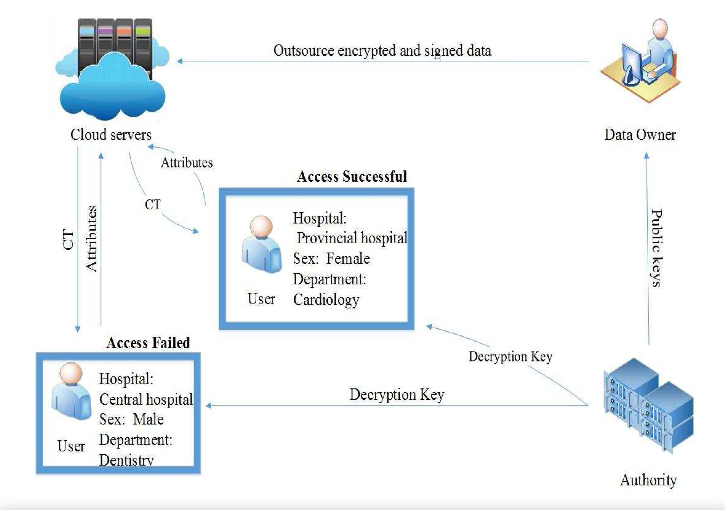
\includegraphics[width=\linewidth]{/Users/tanglixinran/Downloads/河海大学/11.2周六课汇报/fig/Zhang右.png}
            \caption{访问控制示例}
        \end{figure}
    \end{columns}

\end{frame}

\begin{frame}{问题与相关工作}
    \footnotesize  % 使用较小字体

    % 顶部的文字说明
    Koya等人为国外网络节点开发了一种基于生物特征数据的身份验证模型。这是一种混合方案,将一种认证协议与患者的ECG信号相结合。为了提高认证过程,作者从ECG信号中提取生物密钥。这为医疗保健认证系统提供了更好的安全性。该方案可以抵御密钥托管问题和物联网设备模拟攻击。但是,它无法抵抗重放攻击和不可追溯性问题。

    % 两张图片并排放置
    \vspace{0.5cm}  % 调整文字和图片之间的间距
    \begin{columns}
        \column{0.5\textwidth}
        \begin{figure}
            \centering
            \includegraphics[width=\linewidth]{/Users/tanglixinran/Downloads/河海大学/11.2周六课汇报/fig/Koya左.png}
            \caption{系统模型}
        \end{figure}

        \column{0.5\textwidth}
        \begin{figure}
            \centering
            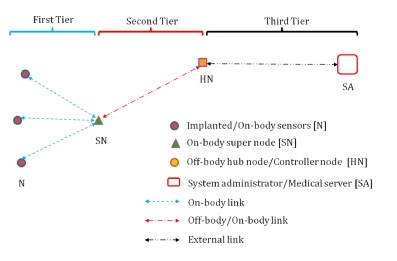
\includegraphics[width=\linewidth]{/Users/tanglixinran/Downloads/河海大学/11.2周六课汇报/fig/Koya右.png}
            \caption{访问控制示例}
        \end{figure}
    \end{columns}

\end{frame}

\begin{frame}{问题与相关工作}
    \footnotesize  % 使用较小字体

    % 顶部的文字说明
    Gupta等人提出了另一种认证模型来改进Koya等人的方案。在这个方案中,他们使用简单的XOR和哈希操作设计了一个安全的密钥协议和匿名身份验证协议。该方案还具有一个动态节点更新过程,可以动态地将新的传感器节点添加到网络中。但研究发现,该方案由于计算成本高、通信开销大,面临可扩展性问题,且无法抵抗去同步攻击。

    % 两张图片并排放置
    \vspace{0.5cm}  % 调整文字和图片之间的间距
    \begin{columns}
        \column{0.5\textwidth}
        \begin{figure}
            \centering
            \includegraphics[width=\linewidth]{/Users/tanglixinran/Downloads/河海大学/11.2周六课汇报/fig/Gupta左.png}
            \caption{系统模型}
        \end{figure}

        \column{0.5\textwidth}
        \begin{figure}
            \centering
            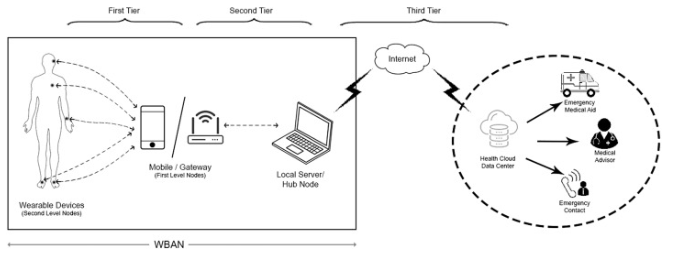
\includegraphics[width=\linewidth]{/Users/tanglixinran/Downloads/河海大学/11.2周六课汇报/fig/Gupta右.png}
            \caption{访问控制示例}
        \end{figure}
    \end{columns}

\end{frame}

\begin{frame}{问题与相关工作}
    \footnotesize  % 使用较小字体

    Farash等人提出了一种\textbf{用户认证和密钥建立方案}。当用户请求在自身和网络内的传感器设备之间建立通信通道时,系统与该特定设备进行通信,并指示该设备执行身份验证过程。然后,在传感器设备和用户之间通过可信网络设备开始身份验证过程。此外,该方案\textbf{使用简单的对称密码学},使整个系统轻量级。遗憾的是,\textbf{该方案无法抵抗某些加密攻击}。尽管许多研究人员在文献中针对不同领域提出了不同的隐私保护、身份验证和访问控制技术,但\textbf{设计一种低资源消耗和高效率的技术仍然具有很高的挑战性}。

    \begin{figure}[htbp]
        \centering
        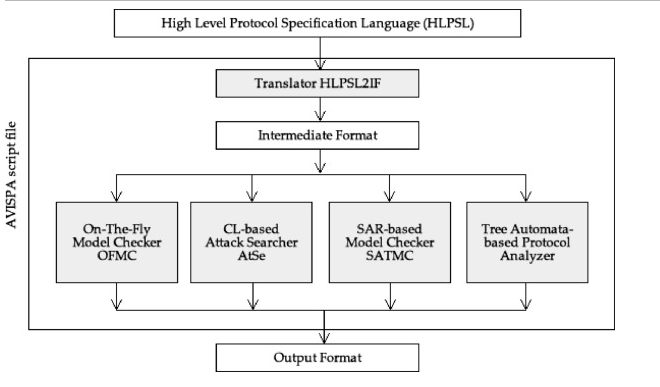
\includegraphics[width=0.6\textwidth]{/Users/tanglixinran/Downloads/河海大学/11.2周六课汇报/fig/Farash.png} % 替换为你的图片路径
        \caption{AVISPA工具的安全验证流程图}
    \end{figure}
\end{frame}


\section{方案构建}

\subsection{系统模型}

\subsubsection{系统模型}
\begin{frame}{系统模型}
    系统模型包括4个主要实体:
    \begin{itemize}
        \item \textbf{物联网设备 (IoT Devices, IoTD)}:与患者身体相关的资源受限设备,用于收集患者的实时医疗数据,并通过网关设备发送给用户。
        \item \textbf{网关 (Gateway):不受资源限制的设备},充当物联网设备与用户之间的中介。
        \item \textbf{中央管理员 (Central Administrator, CA)}:负责初始化系统并对系统中的每个实体进行注册和身份验证。
        \item \textbf{用户 (Users)}:可能是医生或其他医疗工作者,通过网关设备访问物联网设备收集的患者数据。
    \end{itemize}
\end{frame}

\subsubsection{设计目标}
\begin{frame}{设计目标}
    该方案有4个设计目标:
    \begin{itemize}
        \item \textbf{双向认证}:在医疗网络中,设备和用户之间需要相互认证,并同意会话密钥以建立安全通信。
        \item \textbf{消息完整性}:确保医疗数据不会被未授权的用户篡改,从而保障数据的完整性。
        \item \textbf{身份匿名性}:保护用户和设备的身份信息不被攻击者获取和跟踪,防止仿冒攻击和中间人攻击。
        \item \textbf{轻量级设计}:方案必须适合资源受限的物联网设备,使用如XOR和哈希等轻量级操作,以延长设备的使用寿命。
    \end{itemize}
\end{frame}

\subsubsection{威胁模型}
\begin{frame}{威胁模型}
    论文采用了Dolev-Yao安全模型,该模型假设攻击者可以完全控制公共通信信道,并具备以下攻击能力:
    \begin{itemize}
        \item 攻击者可以在不安全信道上拦截、修改、删除或重放消息。
        \item 攻击者可以通过物理攻击获取IoT设备存储的敏感数据。
        \item 攻击者能够进行功率分析攻击来窃取存储在设备内存中的数据。
    \end{itemize}
\end{frame}

\subsection{方案工作流程}
\begin{frame}{方案工作流程}
    \begin{itemize}
        \item 本节介绍了所提出方案的构建过程,包含四个算法,分别为系统初始化、用户注册、设备注册以及登录与认证。
        \item 图\ref{Fig_1}展示了该方案的工作流程。
    \end{itemize}

    \begin{figure}
        \centering
        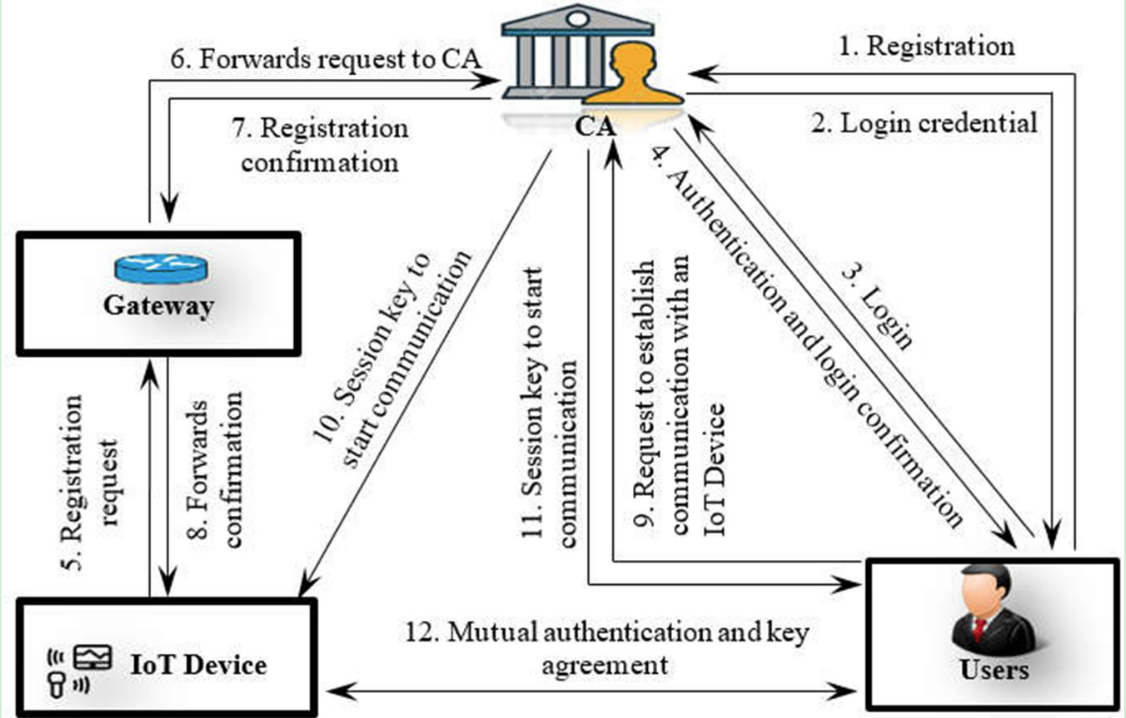
\includegraphics[width=0.7\textwidth]{/Users/tanglixinran/Downloads/河海大学/11.2周六课汇报/fig/Fig_1.png}
        \caption{拟议方案的工作流程}
        \label{Fig_1}
    \end{figure}
\end{frame}

\subsubsection{系统初始化}
\begin{frame}{系统初始化}
    \begin{itemize}
        \item 中央管理员首先通过选择用户、物联网设备 (IoTD) 和网关的密钥值RU、RD和RG来初始化系统。
        \item CA通过安全通道将密钥发送给用户、IoTD和网关。这些密钥会分别安全地存储在各自的内存中。
        \item 图\ref{Fig_2}展示了系统初始化过程。
    \end{itemize}

    \begin{figure}
        \centering
        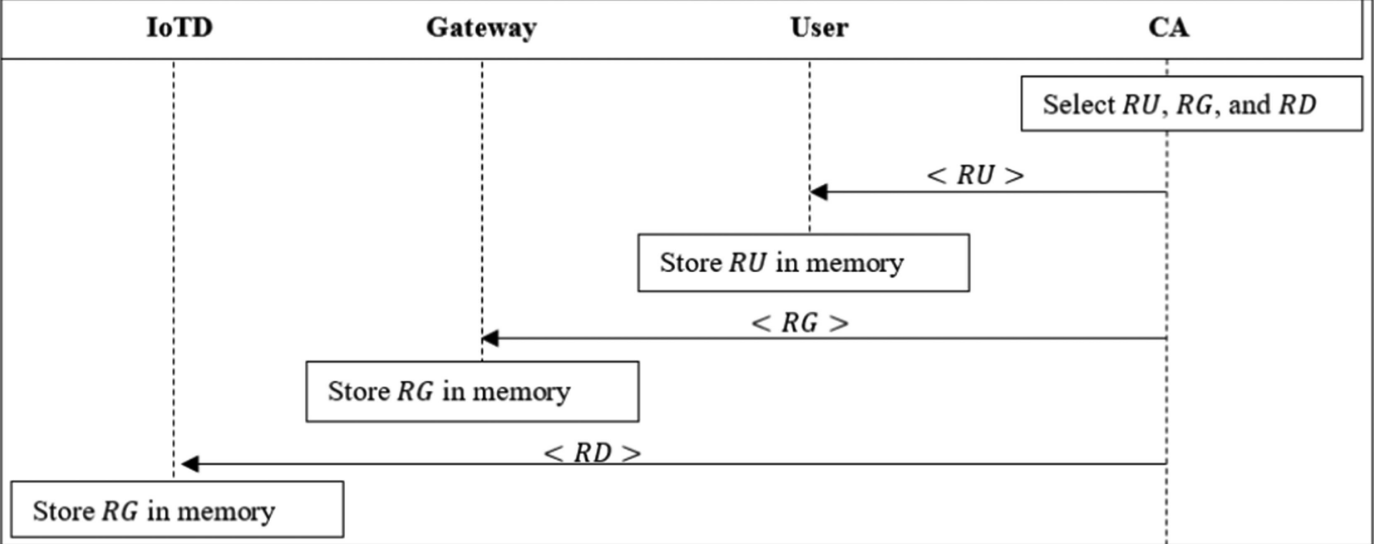
\includegraphics[width=\textwidth]{/Users/tanglixinran/Downloads/河海大学/11.2周六课汇报/fig/Fig_2.png} % 替换为图2的具体文件名
        \vspace{-0.8cm}  % 调整标题和图片之间的距离
        \caption{系统初始化过程}
        \label{Fig_2}
    \end{figure}
\end{frame}

\subsubsection{用户注册}
\begin{frame}{用户注册过程}
    \begin{itemize}
        \item 用户需要将其设备与中央管理员 (CA) 注册以实时获取患者的健康数据。
        \item 整个注册过程如图\ref{Fig_3}所示:
    \end{itemize}
       
    \begin{figure}
        \centering
        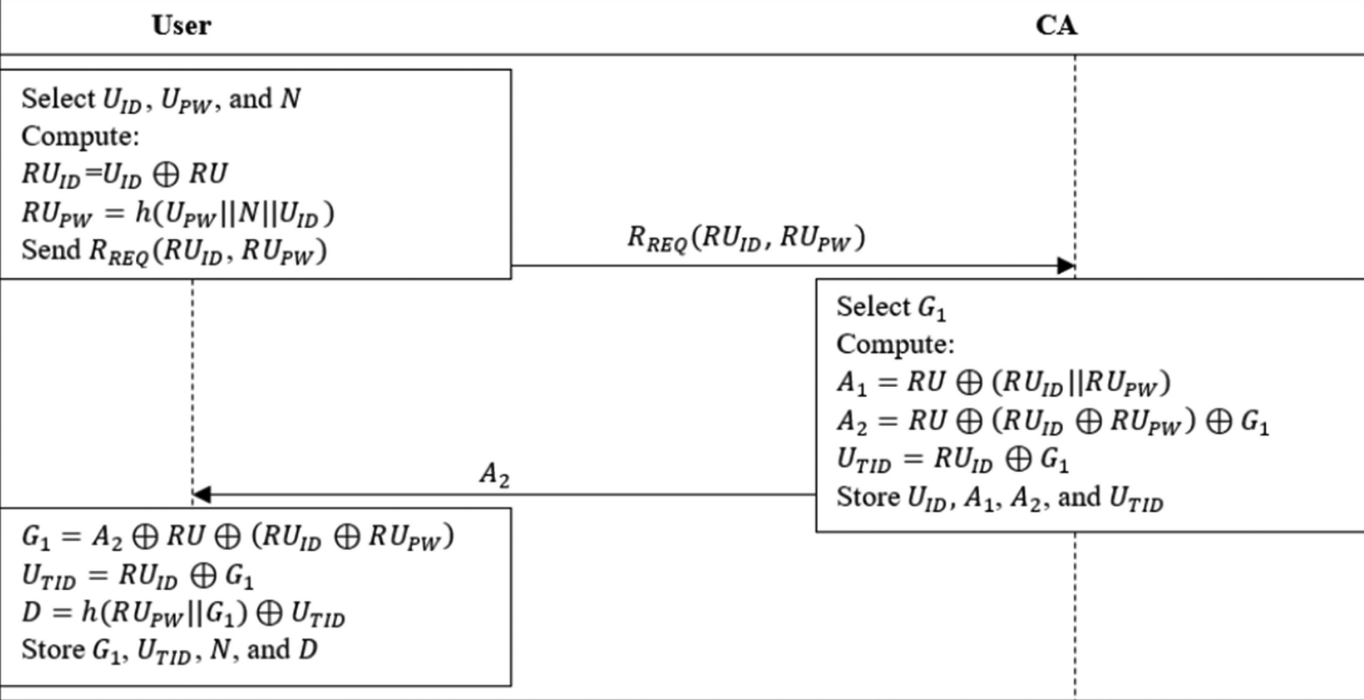
\includegraphics[width=\textwidth]{/Users/tanglixinran/Downloads/河海大学/11.2周六课汇报/fig/Fig_3.png} % 替换为图3的具体文件名
        \caption{用户注册过程}
        \label{Fig_3}
    \end{figure}
\end{frame}



\subsubsection{设备注册}
% 第一页幻灯片
\begin{frame}{设备注册过程}
    \begin{itemize}
        \item 每个物联网设备 (IoTD) 在向用户传输患者的健康数据之前,需要与中央管理员 (CA) 进行注册。
        \item 设备注册过程如图\ref{Fig_4}所示:
    \end{itemize}

    \begin{figure}
        \centering
        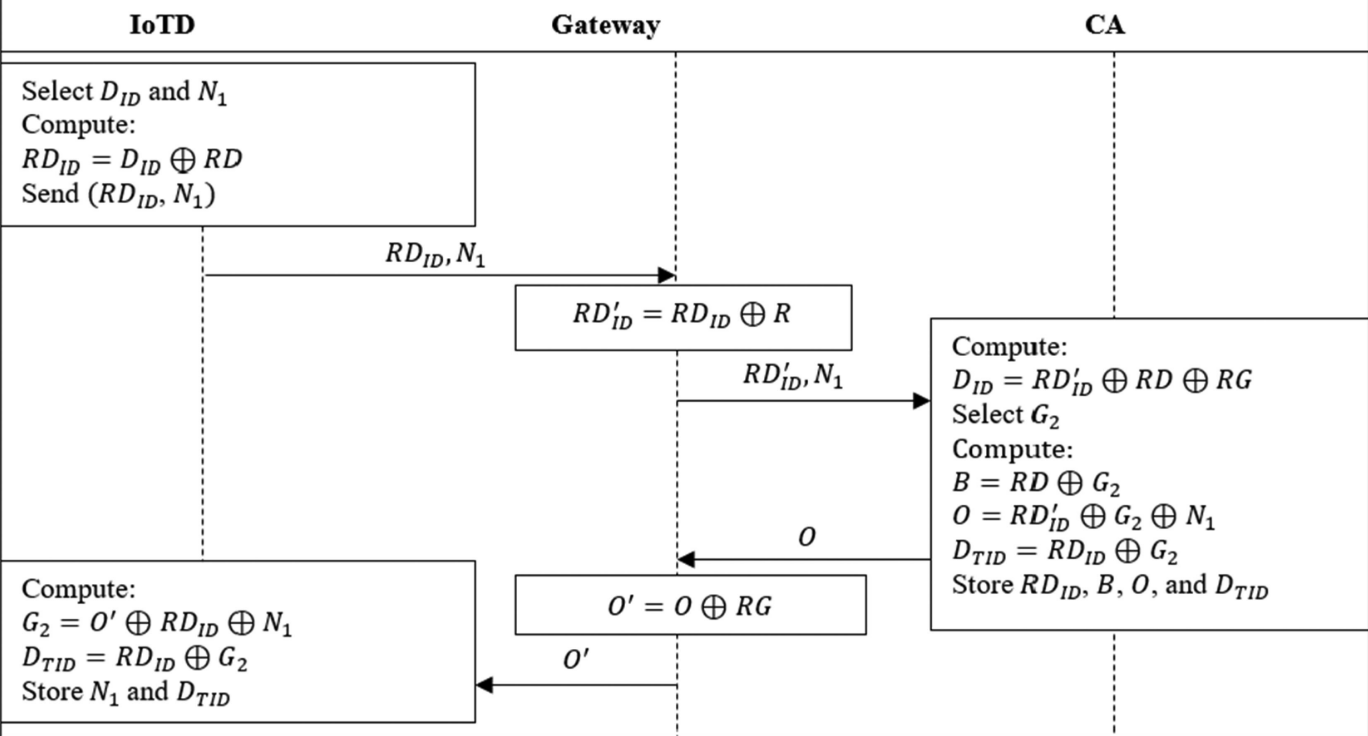
\includegraphics[width=0.9\textwidth]{/Users/tanglixinran/Downloads/河海大学/11.2周六课汇报/fig/Fig_4.png} % 替换为图4的具体文件名
        \vspace{-0.3cm}  % 调整标题和图片之间的距离
        \caption{设备注册过程}
        \label{Fig_4}
    \end{figure}
\end{frame}


\subsubsection{登陆与认证}
% 第一页幻灯片
\begin{frame}{登录与认证过程 (1/2)}
    \begin{itemize}
        \item 该部分展示了用户和物联网设备 (IoTD) 之间的登录和相互认证过程,用户需要通过CA和网关进行身份认证。
        \item 登录和认证过程如图\ref{Fig_5}所示:
    \end{itemize}
\end{frame}

\begin{frame}{登录与认证过程 (2/2)}
    \begin{figure}
        \centering
        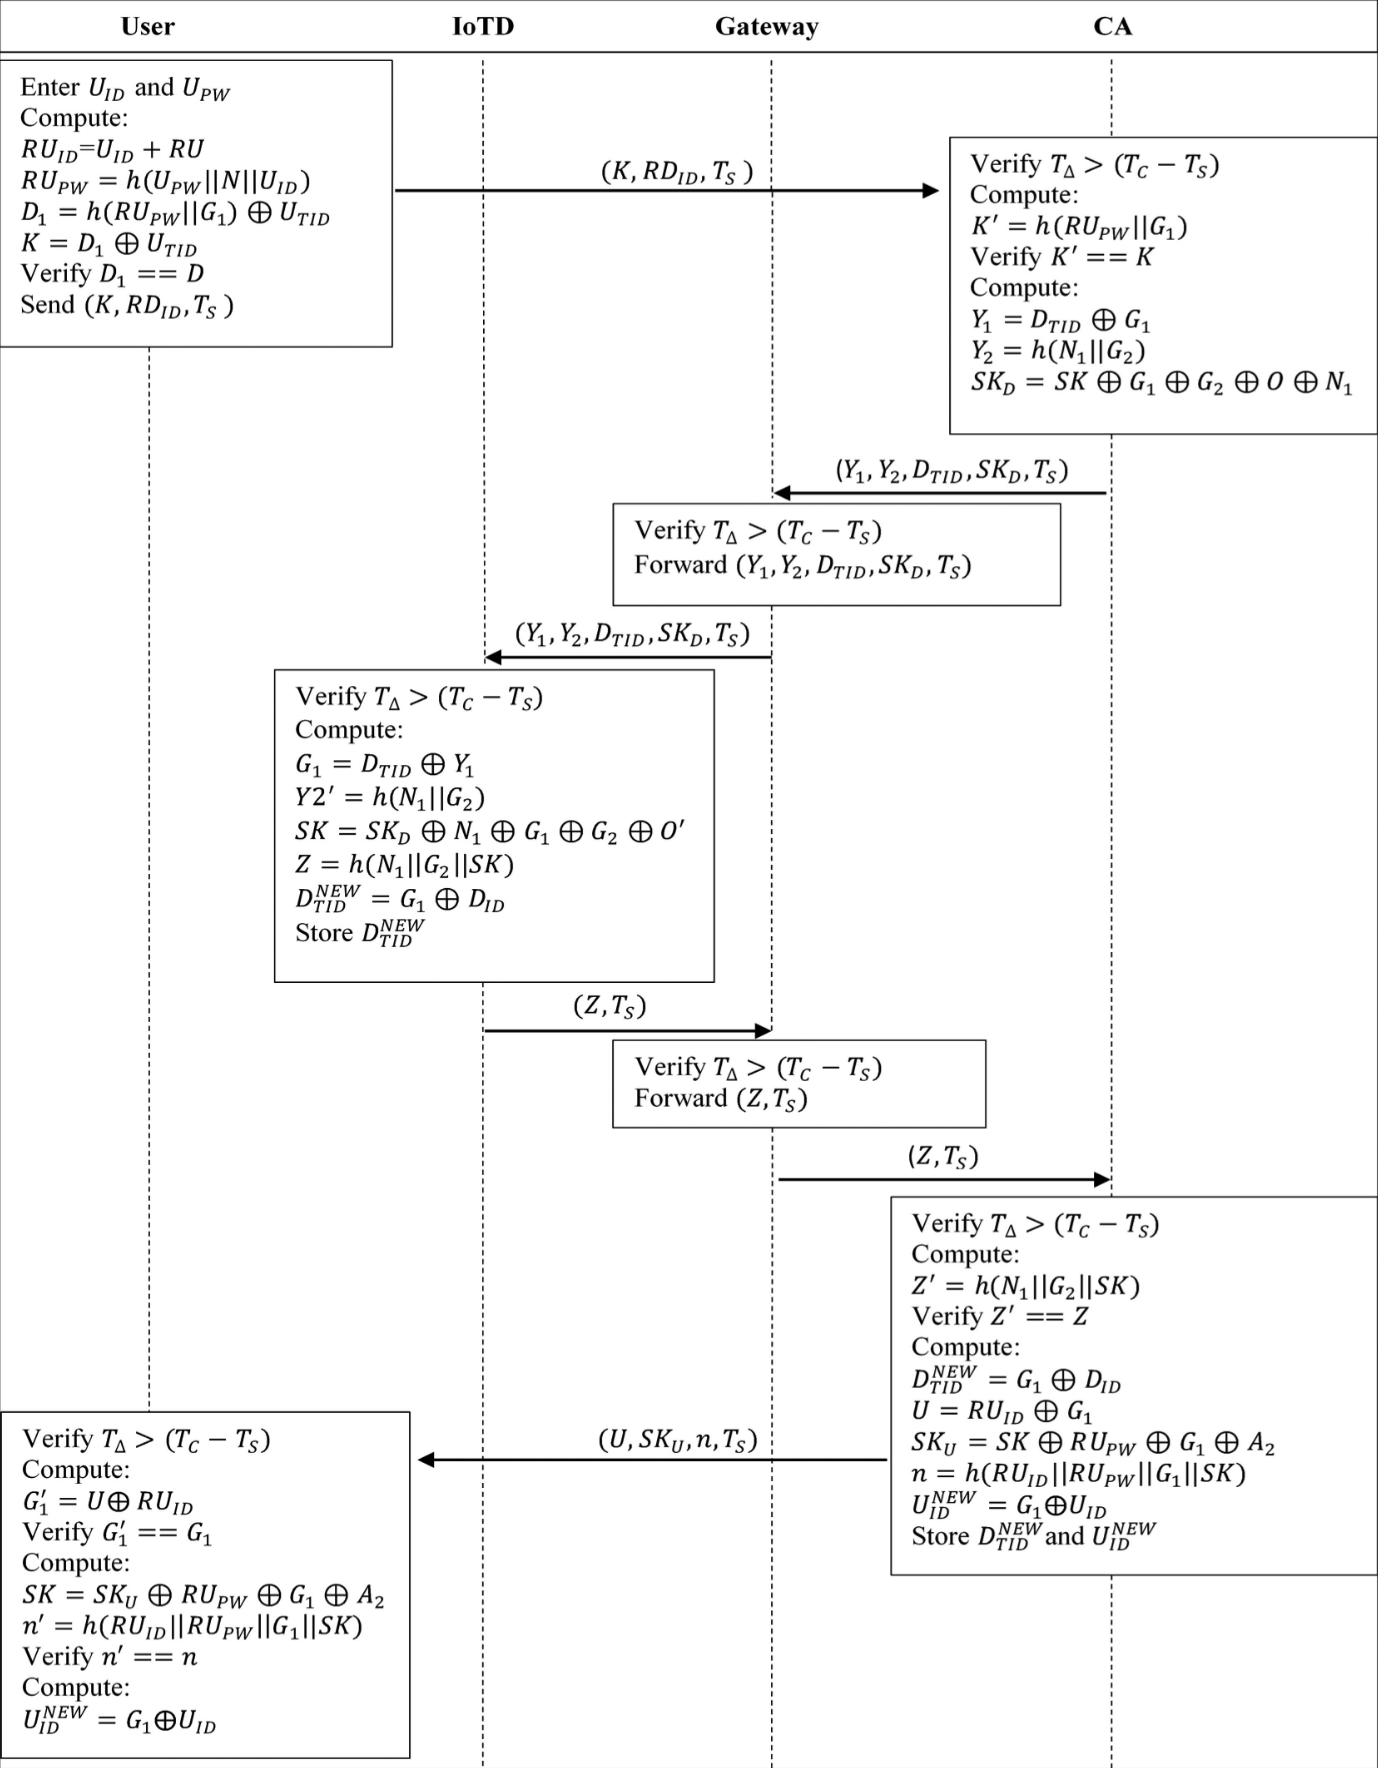
\includegraphics[width=0.5\textwidth]{/Users/tanglixinran/Downloads/河海大学/11.2周六课汇报/fig/Fig_5.png} % 替换为图5的具体文件名
        \vspace{-0.4cm}  % 调整标题和图片之间的距离
        \caption{登录与认证过程}
        \label{Fig_5}
    \end{figure}
\end{frame}

\section{安全与性能分析}
\subsection{安全分析}
\subsubsection{形式分析}
% 第一页:引入ROR模型
\begin{frame}{使用ROR模型的形式化分析 (1/4)}
    \begin{itemize}
        \item 本节介绍通过使用ROR模型对提出方案的安全性进行分析。ROR模型是一种用来验证会话密钥安全性的概率模型。
        \item 假设攻击者\textbf{A}完全控制通信信道,能够捕获、修改、篡改、重定向、删除或重放通过网络发送的所有消息。
        \item 攻击者\textbf{A}可以执行以下查询:
        \begin{itemize}
            \item \textbf{Exe($\xi$)}: 执行窃听攻击,获取有效方之间交换的消息。
            \item \textbf{Snd($\xi$, $\mathcal{M}$)}: 攻击者可以发送消息$\mathcal{M}$给$\xi$,并接收$\xi$的回复。
            \item \textbf{Cpt($\xi$)}: 攻击者可以执行捕获攻击,获取存储在物联网设备(IoTD)、网关和用户设备中的所有参数。
        \end{itemize}
    \end{itemize}
\end{frame}

% 第二页:攻击者的其他查询
\begin{frame}{使用ROR模型的形式化分析 (2/4)}
    \begin{itemize}
        \item 继续介绍攻击者\textbf{A}的查询:
        \begin{itemize}
            \item \textbf{Hsh($S$)}: 攻击者通过此查询获取输入字符串$S$的固定长度哈希值。
            \item \textbf{Tst($\xi$)}: 在此查询中,攻击者随机选择一个会话密钥($SK$),如果$c=1$,攻击者获取真实的$SK$;如果$c=0$,获取随机数。
        \end{itemize}
        \item \textbf{A}赢得游戏的事件称为\textbf{Suc},并且\textbf{A}破坏方案的优势定义为:
        \[
        Adv^\xi_{\mathcal{A}} = |2Prob(Suc) - 1|
        \]
    \end{itemize}
\end{frame}

% 第三页:展示定理
\begin{frame}{使用ROR模型的形式化分析 (3/4)}
    \begin{theorem}
        对于一个多项式时间$t$内运行的攻击者$\mathcal{A}$,其破坏方案的优势满足:
        \[
\text{Adv}_{\mathcal{A}}^{\xi} \leq 2 \max \left\{ D' \cdot q_{snd}, \frac{q_{snd}}{2^f} \right\} + \frac{q_{snd}}{2^{f-2}} + \frac{3q_{hsh}^2}{2^{f-1}}.
\]
        其中,$D'$ 和 $b$ 是两个常数,$f$ 是用户输入信息的长度。
    \end{theorem}
    
    \begin{itemize}
        \item 证明使用六个游戏序列来展示。每个游戏$G_i$都计算了攻击者\textbf{A}在不同查询规则下的成功概率。
    \end{itemize}
\end{frame}

% 第四页:展示具体推导步骤
\begin{frame}{使用ROR模型的形式化分析 (4/4)}
    \begin{itemize}
        \item 从$G_0$到$G_6$,展示了攻击者\textbf{A}的各种攻击行为对破坏方案的成功概率影响,结果是每个游戏的成功概率不断递减。
        \[
\text{Prob} \left[ \text{Suc}_{\mathcal{A}}^{G_6} \right] - \text{Prob} \left[ \text{Suc}_{\mathcal{A}}^{G_5} \right] \leq \frac{q_{hsh}^2}{2^{f+1}}.
\]
        最终得出:
        \[
\text{Adv}^{\xi}_{\mathcal{A}} \leq 2 \max \left\{ D' \cdot q_{snd}^{b}, \frac{q_{snd}}{2^f} \right\} + \frac{q_{snd}}{2^{f-2}} + \frac{3q_{hsh}^2}{2^{f-1}}.
\]
    \end{itemize}
\end{frame}

% 第一页幻灯片
\begin{frame}{使用AVISPA工具的形式化分析 (1/2)}
    \begin{itemize}
        \item 本节展示了使用AVISPA工具对提出的方案进行形式化验证。AVISPA工具是一种自动化的形式化验证工具,用于分析协议的安全性。
        \item AVISPA使用高级协议规范语言 (HLPSL) 描述协议,并通过转换器 (HLPSL2IF) 将其转换为中间格式 (IF),然后使用工具的四个后端进行分析:
        \begin{itemize}
            \item 基于安全协议分析的树自动机 (TA4SP)
            \item 基于约束逻辑的攻击搜索 (CL-AtSe)
            \item 基于SAT的模型检查器 (SATMC)
            \item 基于在线模型检查的OFMC
        \end{itemize}
        \item 结果显示协议的安全或不安全状态。
    \end{itemize}
\end{frame}

% 第二页幻灯片
\begin{frame}{使用AVISPA工具的形式化分析 (2/2)}
    \begin{itemize}
        \item 提出的方案的HLPSL代码使用AVISPA工具的Security Animator (SPAN)模拟工具进行分析。分析结果如图\ref{Fig_6}所示。
        \item 该分析显示,方案在CL-AtSe和OFMC后端上都是安全的,能够抵御已知攻击,且会话密钥的机密性得到了验证。
    \end{itemize}

    \begin{figure}
        \centering
        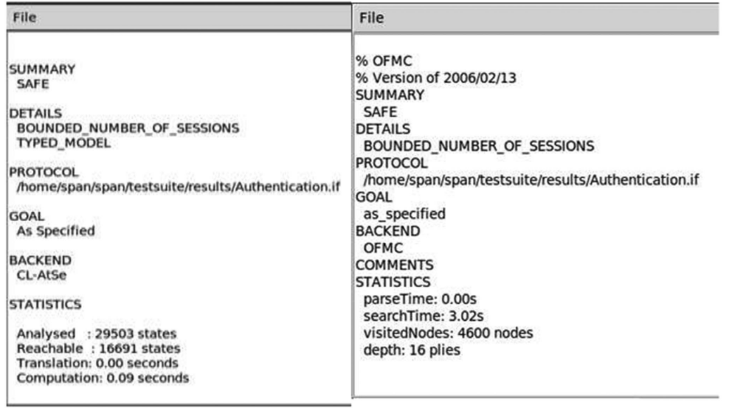
\includegraphics[width=0.7\textwidth]{/Users/tanglixinran/Downloads/河海大学/11.2周六课汇报/fig/Fig_6.png} % 替换为图6的具体文件名
        \caption{AVISPA工具生成的输出结果}
        \label{Fig_6}
    \end{figure}
\end{frame}

\subsubsection{非正式分析}
% 第一页幻灯片:窃听攻击与重放攻击
\begin{frame}{非正式分析 (1/2)}
    \begin{itemize}
        \item 提出的方案能够抵御多种攻击,如窃听攻击、重放攻击、特权内部攻击以及被盗凭证攻击。该方案还保持了匿名性和不可追踪性。
        
        \item \textbf{窃听攻击}:在窃听攻击中,攻击者\textbf{A}可以截获、删除或修改传输的数据。即使攻击者获取了所有传输的消息,也无法获得会话密钥,因为\textbf{A}不知道\textit{G1} 和 \textit{G2},以及CA在注册过程中选择的密钥值 \textit{RD}、\textit{RU} 和 \textit{RG}。
        
        \item \textbf{重放攻击}:在重放攻击中,攻击者通过重放之前会话中的消息来获得网络访问权限。提出的方案通过使用时间戳来防止这种攻击,确保消息在有效的传输延迟范围内被处理。
    \end{itemize}
\end{frame}

% 第二页幻灯片:特权内部攻击、被盗验证攻击、匿名性与不可追踪性
\begin{frame}{非正式分析 (2/2)}
    \begin{itemize}
        \item \textbf{特权内部攻击}:在这种攻击中,内部攻击者可能获取到用户的身份和密码。然而,由于\textit{A2} 使用密钥值\textit{RU}加密,且攻击者不知道\textit{RU} 和 \textit{G1},因此攻击者无法计算出会话密钥。
        
        \item \textbf{被盗验证攻击}:在这种攻击中,攻击者通过获取某些节点的验证凭证尝试计算会话密钥。但由于\textbf{A}无法获取\textit{RU},无法成功计算出用户的身份和会话密钥,从而抵御被盗验证攻击。
        
        \item \textbf{匿名性与不可追踪性}:提出的方案确保用户的真实身份\textit{UID}不会被攻击者获取,且用户的活动不会被追踪。即使攻击者获取了\textit{RUID} 和 \textit{RUPW},也无法通过这些信息追踪到用户。
    \end{itemize}
\end{frame}

\subsection{性能分析}
% 第一页:安全特性比较
\subsubsection{安全特性比较}
\begin{frame}{安全特性比较}
    \begin{itemize}
        \item 表\ref{table:2}显示了提出的方案与其他方案在安全特性方面的比较,包括抵抗特权内部攻击、离线密码猜测、MITM攻击、以及IoTD伪装等。
    \end{itemize}
    \begin{table}[ht]
        \centering
        % 使用 \resizebox 将表格调整为合适的宽度
        \resizebox{\textwidth}{!}{
        \begin{tabular}{lccccccc}  
            \toprule
            \textbf{方案} & \textbf{特权内部攻击} & \textbf{离线密码猜测} & \textbf{前向保密性} & \textbf{MITM攻击} & \textbf{IoTD伪装} & \textbf{IoTD捕获} & \textbf{被盗验证攻击} \\
            \midrule
            \textbf{[30]} & Y & N & N & N & Y & Y & Y \\
            \textbf{[32]} & N & Y & N & Y & N & N & N \\
            \textbf{[33]} & N & Y & N & Y & N & N & N \\
            \textbf{[34]} & Y & Y & Y & Y & Y & N & N \\
            \textbf{提出方案} & Y & Y & Y & Y & Y & Y & Y \\
            \bottomrule
        \end{tabular}
        }
        \caption{不同方案的安全特性比较}
        \label{table:2}
    \end{table}
\end{frame}

% 第二页:存储需求比较
\subsubsection{存储成本比较}
\begin{frame}{存储需求比较}
    \begin{itemize}
        \item 提出的方案使用SHA-256哈希操作,其密钥长度为256位。
        \item 表\ref{table:3}显示了不同方案在各个实体的存储需求比较。
    \end{itemize}

    % 存储成本比较表格
    \begin{table}[ht]
        \centering
        % 使用 \resizebox 将表格调整为合适的宽度
        \resizebox{\textwidth}{!}{
        \begin{tabular}{lccccc}  
            \toprule
            \textbf{Scheme} & \textbf{User} & \textbf{IoTD} & \textbf{IN} & \textbf{CA} & \textbf{Total} \\
            \midrule
            \textbf{[30]} & 1088b & - & 992b & 160b & 2240b \\
            \textbf{[32]} & 576b & 576b & 640b & 1792b & 2944b \\
            \textbf{[33]} & - & 640b & 640b & 480b & 1780b \\
            \textbf{[34]} & - & 1088b & 320b & 320b & 1728b \\
            \textbf{Proposed scheme} & 736b & 320b & 160b & 1216b & 2432b \\
            \bottomrule
        \end{tabular}
        }
        \caption{Proposed Scheme's Storage Cost in Bits (b)}
        \label{table:3}
    \end{table}
\end{frame}

\subsubsection{计算成本比较}
% 第三页:计算成本比较 - 表4
\begin{frame}{计算成本比较 (1/2)}
    \begin{itemize}
        \item 表\ref{table:4}展示了不同方案在用户注册、设备注册、登录和认证阶段的计算成本。
        \item 哈希操作的总时间也列在表中。
    \end{itemize}

    % 计算成本比较表格 (Table 4)
    \begin{table}[ht]
        \centering
        % 使用 \resizebox 调整表格宽度以适应页面
        \resizebox{\textwidth}{!}{
        \begin{tabular}{lccccc}  
            \toprule
            \textbf{Phase} & \textbf{User} & \textbf{IoTD} & \textbf{CA} & \textbf{Total} & \textbf{Total Time (ms)} \\
            \midrule
            User registration & 2H$_{CC}$ & - & - & 2H$_{CC}$ & 0.0008 \\
            Device registration & - & - & - & - & - \\
            Login and authentication & 3H$_{CC}$ & 2H$_{CC}$ & 4H$_{CC}$ & 9H$_{CC}$ & 0.0036 \\
            \textbf{Total cost} & \textbf{5H$_{CC}$} & \textbf{2H$_{CC}$} & \textbf{4H$_{CC}$} & \textbf{11H$_{CC}$} & \textbf{0.0044} \\
            \bottomrule
        \end{tabular}
        }
        \caption{Proposed Scheme's Computation Cost in Different Phases}
        \label{table:4}
    \end{table}
\end{frame}

% 第四页:计算成本比较 - 表5
\begin{frame}{计算成本比较 (2/2)}
    \begin{itemize}
        \item 表\ref{table:5}展示了不同方案在计算成本上的比较,提出的方案表现出较优的计算效率。
    \end{itemize}

    % 计算成本比较表格 (Table 5)
    \begin{table}[ht]
        \centering
        % 使用 \resizebox 调整表格宽度以适应页面
        \resizebox{\textwidth}{!}{
        \begin{tabular}{lccccc}  
            \toprule
            \textbf{Scheme} & \textbf{User} & \textbf{IoTD} & \textbf{CA} & \textbf{Total} & \textbf{Time (ms)} \\
            \midrule
            \textbf{[30]} & 10H$_{CC}$ & 19H$_{CC}$ & 7H$_{CC}$ & 36H$_{CC}$ & 0.0144 \\
            \textbf{[32]} & 3H$_{CC}$ & 2H$_{CC}$ & 3H$_{CC}$ & 8H$_{CC}$ & 0.0032 \\
            \textbf{[33]} & - & 3H$_{CC}$ & 10H$_{CC}$ & 13H$_{CC}$ & 0.0052 \\
            \textbf{[34]} & - & 7H$_{CC}$ & 10H$_{CC}$ & 17H$_{CC}$ & 0.0068 \\
            \textbf{Proposed scheme} & 2H$_{CC}$ & 3H$_{CC}$ & 4H$_{CC}$ & 9H$_{CC}$ & 0.0036 \\
            \bottomrule
        \end{tabular}
        }
        \caption{Comparison of Computation Cost}
        \label{table:5}
    \end{table}
\end{frame}

\subsubsection{通信成本比较}
% 第五.1页:通信成本比较
\begin{frame}{通信成本比较}
    \begin{itemize}
        \item 表\ref{table:6}展示了不同方案在消息交换数量和总比特数上的通信成本比较。
        \item 提出的方案表现出较好的通信效率,特别是在消息交换数量与比特数的平衡方面。
    \end{itemize}

    % 通信成本比较表格 (Table 5)
    \begin{table}[ht]
        \centering
        \resizebox{\textwidth}{!}{
        \begin{tabular}{lcc}  
            \toprule
            \textbf{Scheme} & \textbf{No. of message exchanged} & \textbf{Total no. of bits} \\
            \midrule
            \textbf{[30]} & 4 & 3840 \\
            \textbf{[32]} & 4 & 1024 \\
            \textbf{[33]} & 6 & 5376 \\
            \textbf{[34]} & 4 & 4096 \\
            \textbf{Proposed scheme} & 6 & 1536 \\
            \bottomrule
        \end{tabular}
        }
        \caption{Comparison of Communication Cost}
        \label{table:6}
    \end{table}
\end{frame}
% 第五.2:图7
\begin{frame}{执行时间比较}
    \begin{itemize}
        \item 图\ref{Fig_7}展示了不同方案在用户注册、设备注册、以及认证阶段的执行时间比较。
        \item 提出的方案在这些阶段的执行时间相对较短,表明其具有较好的性能表现。
    \end{itemize}

    % 插入图7
    \begin{figure}[ht]
        \centering
        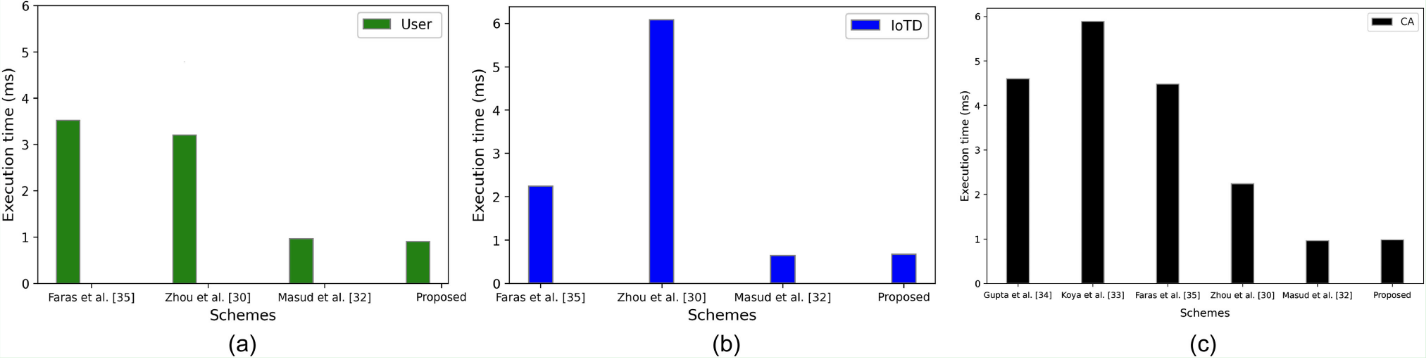
\includegraphics[width=\textwidth]{/Users/tanglixinran/Downloads/河海大学/11.2周六课汇报/fig/Fig_7.png}  % 修改为图7的路径
        \caption{Comparisons of execution time (a) User registration, (b) Device registration, and (c) Authentication phase}
        \label{Fig_7}
    \end{figure}
\end{frame}

\section{总结}
% 结论与未来工作 幻灯片
\begin{frame}{结论与未来工作}
    \begin{itemize}
        \item 本文提出了一种基于简单加密操作的轻量级用户与设备认证方案,能够保证用户匿名性,并抵抗多种密码学攻击。
        \item 安全性和性能分析验证了方案的有效性和效率,该方案在注册时间和认证时间上优于许多现有方案。
        \item 未来工作可通过改进方案的开销问题,并为物联网医疗应用引入多因素认证机制。
    \end{itemize}
\end{frame}
















\begin{frame}
    \begin{center}
        {\Huge\calligra 感谢大家的聆听}
    \end{center}
\end{frame}


\end{document}